\section{Problemas}

% \begin{figure}[H]
%   \centering
%   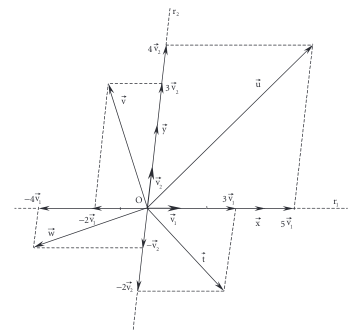
\includegraphics[width=0.6\textwidth]{./fig/fig1.38.png}
%   \caption{Vetores expressos em $\vec{v_1}$ e $\vec{v_2}$}\label{fig:fig1.38}
% \end{figure}

\question{
  Dados os vetores $\vec{u} = 2\vec{i} - 3\vec{j}$, $\vec{v} = \vec{i} -
    \vec{j}$ e $\vec{w} = -2\vec{i} + \vec{j}$, determinar:
}
\begin{itemize}
  \item \subquestion{$2\vec{u} - \vec{v}$}
  \answer{
    \begin{align*}
    2\vec{u} &= 2(2\vec{i} - 3\vec{j}) = 4\vec{i} - 6\vec{j} \\
      2\vec{u} - \vec{v} &= (4\vec{i} - 6\vec{j}) - (\vec{i} - \vec{j}) \\
      &= 4\vec{i} - 6\vec{j} - \vec{i} + \vec{j} \\
      &= (4 - 1)\vec{i} + (-6 + 1)\vec{j} \\
      &= 3\vec{i} - 5\vec{j} \\
      \end{align*}
  }
  
  \item \subquestion{$\vec{v} - \vec{u} + 2\vec{w}$}
  \answer{
    \begin{align*}
    \vec{v} &= \vec{i} - \vec{j} \\
      -\vec{u} &= - (2\vec{i} - 3\vec{j}) = -2\vec{i} + 3\vec{j} \\
      2\vec{w} &= 2(-2\vec{i} + \vec{j}) = -4\vec{i} + 2\vec{j} \\
      \vec{v} - \vec{u} + 2\vec{w} &= (\vec{i} - \vec{j}) + (-2\vec{i} + 3\vec{j}) + (-4\vec{i} + 2\vec{j}) \\
      &= (\vec{i} - 2\vec{i} - 4\vec{i}) + (-\vec{j} + 3\vec{j} + 2\vec{j}) \\
      &= -5\vec{i} + 4\vec{j} \\
      \end{align*}
  }
  
  \item \subquestion{$\frac{1}{2}\vec{u} - 2\vec{v} - \vec{w}$}
  \answer{
    \begin{align*}
    \frac{1}{2}\vec{u} &= \frac{1}{2}(2\vec{i} - 3\vec{j}) = \vec{i} - \frac{3}{2}\vec{j} \\
      -2\vec{v} &= -2(\vec{i} - \vec{j}) = -2\vec{i} + 2\vec{j} \\
      -\vec{w} &= -(-2\vec{i} + \vec{j}) = 2\vec{i} - \vec{j} \\
      \frac{1}{2}\vec{u} - 2\vec{v} - \vec{w} &= (\vec{i} - \frac{3}{2}\vec{j}) + (-2\vec{i} + 2\vec{j}) + (2\vec{i} - \vec{j}) \\
      &= (\vec{i} - 2\vec{i} + 2\vec{i}) + \left(-\frac{3}{2}\vec{j} + 2\vec{j} - \vec{j}\right) \\
      &= \vec{i} + \left(-\frac{3}{2} + 2 - 1\right)\vec{j} \\
      &= \vec{i} - \frac{1}{2}\vec{j} \\
      \end{align*}
  }
  
  \item \subquestion{$3\vec{u} - \frac{1}{2}\vec{v} - \frac{1}{2}\vec{w}$}
  \answer{
    \begin{align*}
    3\vec{u} &= 3(2\vec{i} - 3\vec{j}) = 6\vec{i} - 9\vec{j} \\
      \frac{1}{2}\vec{v} &= \frac{1}{2}(\vec{i} - \vec{j}) = \frac{1}{2}\vec{i} - \frac{1}{2}\vec{j} \\
      \frac{1}{2}\vec{w} &= \frac{1}{2}(-2\vec{i} + \vec{j}) = -\vec{i} + \frac{1}{2}\vec{j} \\
      3\vec{u} - \frac{1}{2}\vec{v} - \frac{1}{2}\vec{w} &= (6\vec{i} - 9\vec{j}) - \left(\frac{1}{2}\vec{i} - \frac{1}{2}\vec{j}\right) - \left(-\vec{i} + \frac{1}{2}\vec{j}\right) \\
      &= \left(6 - \frac{1}{2} + 1\right)\vec{i} + \left(-9 + \frac{1}{2} - \frac{1}{2}\right)\vec{j} \\
      &= \frac{11}{2}\vec{i} - 9\vec{j} \\
      \end{align*}
  }
\end{itemize}
